\documentclass[a4paper]{article}
\usepackage{amsmath}
\usepackage[T2A]{fontenc}
\usepackage[english, russian]{babel}
\usepackage{mathtools}
\usepackage{amsfonts}
\usepackage{graphicx}
\usepackage{wrapfig}

\title{Что-то дифферинцируется, а что-то нет, но это не плохо)}
\author{Владимир Швабра}
\date{\today}
\begin{document}
\maketitle
\newpage

\subsection{Исходная функция:}

$$
\left(\sin{x}+{2}\right)\cdot{2^{0-{x^{2}}}}
$$
\subsection{Упростим её:}

$$
\left(\sin{x}+{2}\right)\cdot{2^{\left(-1\right)\cdot{x^{2}}}}
$$
\subsection{Получившаяся производная:}

$$
\cos{x}\cdot{2^{\left(-1\right)\cdot{x^{2}}}}+{2\cdot{x}\cdot{\left(-1\right)}\cdot{0,693147\cdot{2^{\left(-1\right)\cdot{x^{2}}}}}\cdot{\left(\sin{x}+{2}\right)}}
$$
\subsection{Упростим её:}

$$
\cos{x}\cdot{2^{\left(-1\right)\cdot{x^{2}}}}+{2\cdot{x}\cdot{\left(-1\right)}\cdot{0,693147\cdot{2^{\left(-1\right)\cdot{x^{2}}}}}\cdot{\left(\sin{x}+{2}\right)}}
$$
\subsection{Графики:}

\begin{figure}[h]
\centering
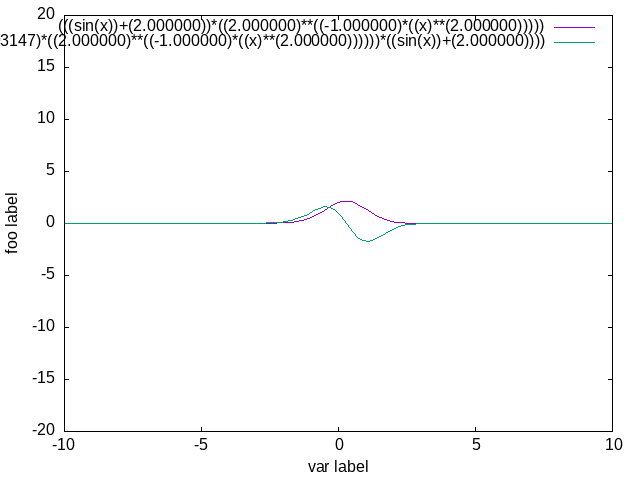
\includegraphics[width=0.8\linewidth]{assets/input.tex_graphic.png}
\end{figure}

\end{document}